\subsubsection{Memory Intensive}
\label{section:perf-memory}

Last but not least, we will examine the performance of the SUTs when executing memory intensive program; the test suite \texttt{memcpyw(n)} copies \texttt{n} words (each of which is 4 bytes) from one memory location to another. Not only does this involve very frequent memory instructions, it also causes large amounts of memory to be touched in the memory map for large \texttt{n}.

\begin{figure}[H]
    \centering
    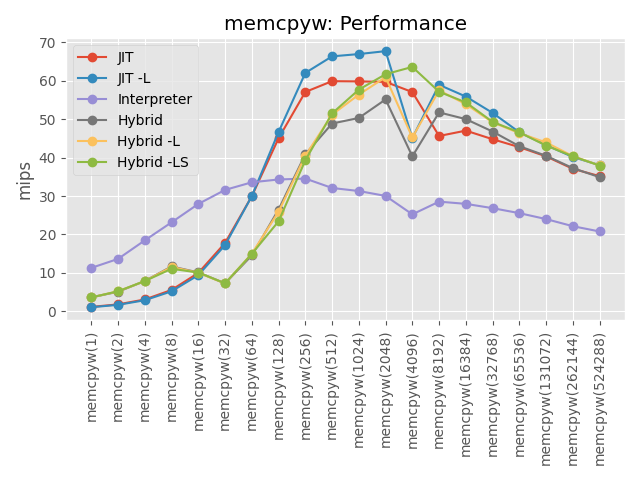
\includegraphics[scale=0.75]{output/graphs/tests/all/memcpyw/mips.png}
    \caption{Performance in mips of the memcpyw test suite.}
    \label{figure:memcpyw-mips}
\end{figure}

The performance for the test suite is shown in \autoref{figure:memcpyw-mips}; unlike most test suites which show monotonic performance with \texttt{n}, all SUTs experienced a parabolic relationship with \texttt{n} where the performance rapidly rose to a peak before falling again. This may seem confusing, as higher \texttt{n} results in hotter blocks, which we have established results in higher performance. The answer becomes clear however when we acknowledge that increased \texttt{n} also causes a larger footprint of emulated memory.

This is because the more memory copied by the test, the more insertions and accesses are made to the internal hash table powering the memory map. Insertion and access time for the map implementation used becomes slower the more items present in the map \cite{tessil-benchmark}. This linear slowdown is true for all other major C++ unordered map implementations \cite{tessil-benchmark}. This slowdown affects both SUTs as they both internally use the same memory map.

Since large \texttt{n} increased performance due to hotness, but decreases performance due to memory map congestion, the two factors oppose each other, and we are left with a performance sweet spot where the combined overhead is minimised. We can see that this sweet spot moves further to right the more the emulator benefits from program hotness by comparing the curve to \texttt{JIT -L} to the interpreter: in the case of \texttt{JIT -L}, the sweet spot occurs at $n\approx2048$, yet for the interpreter it is much lower at only $n\approx256$.

Moreover, the peak performance of all emulators is significantly lower in this test suite than the other test suites covered previously; regardless of program hotness or the emulator used, memory instructions are slow to emulate due to the memory map implementation and result in universally poor performance. This said, the JIT and hybrid emulators are still able to outperform the interpreter and the typical performance pecking order is maintained.

\begin{figure}[H]
    \centering
    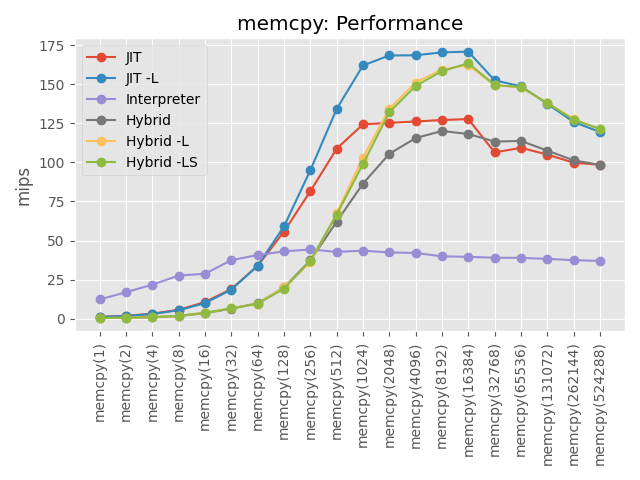
\includegraphics[scale=0.75]{output/graphs/tests/all/memcpy/mips.png}
    \caption{Performance in mips of the memcpy test suite.}
    \label{figure:memcpy-mips}
\end{figure}

Another test suite of interest is \texttt{memcpy(n)}, the performance of which is shown in \autoref{figure:memcpy-mips}. \texttt{memcpy(n)} copies \texttt{n} bytes of memory instead of \texttt{n} words.

On a real MIPS system, we might expect that \texttt{memcpy(n)} would perform worse. This is because the reads and writes are no longer word aligned which typically results in lower performance. As is obvious, this was not the case under the emulation. Despite the added complexity and overhead required with non-word-aligned, sub-word memory accesses, the fact that the emulated memory footprint is $4\times$ smaller made up for it. Since the memory map stores entries at the word level, 4 contiguous bytes are stored in a single entry. This reduced congestion increases the performance of the hash table allowing \texttt{memcpy(n)} to outperform \texttt{memcpyw(n)}.

To conclude, despite being able to outperform the interpreter in memory intensive workloads, neither the JIT nor hybrid are able to perform particularly well due to the slow memory map.